\glsresetall{} 


\chapter{Software Workflow}\label{chap:workflow}

To demonstrate how \gls{pops} may be used, let us walk through setting up
\gls{pops} for the EG-SAT mission. Suppose the customer defines an Area Target
AOI in the Norwegian Sea where they wish Coarse Imaging and Tip-and-Cue Imaging
to be performed. The \gls{aoi} is defined by the points  in
Table~\ref{tab:norway-aoi}. It is the operator’s responsibility to construct an
operations plan for the next week. To do this, they may use \gls{pops} to aid
them in laying out the deterministic aspects of an operations plan.  That
being, determining remote-sensing opportunities, creating a schedule of
observations, validating that schedule, and creating \glspl{ttc} to be uploaded
to the spacecraft. It should be noted that the real-time ground processing of
the data and the generation of new \glspl{ttc} for the next pass of the
Tip-and-Cue Mode are beyond the capabilities of \gls{pops} and this is handled
by separate, mission-specific automatic ground processing.

\begin{table}[h] 
    \centering
    \caption{Area of Interest Definition}
    \begin{tabular}{cccc}
	Point                  & Latitude [$^\circ$] & Longitude [$^\circ$] & Altitude [m] \\ \hline
	\multicolumn{1}{l|}{0} & 73       & -20      & 0        \\
	\multicolumn{1}{l|}{1} & 66       & 19       & 0        \\
	\multicolumn{1}{l|}{2} & 78       & 41       & 0        \\
	\multicolumn{1}{l|}{3} & 82       & 9        & 0        \\
	\multicolumn{1}{l|}{4} & 79       & -17      & 0       
    \end{tabular}
    \label{tab:norway-aoi}
\end{table}

Each step in this process makes use of menus and forms in \gls{pops} that a
user can fill out. To avoid having an excessive number of screenshots for each
step, the input data itself will be shown in tables or figures rather than
through screenshots of the menus.

\subsection{Plan Configuration}

First, \gls{pops} must be configured for a particular mission. The operator
must specify the mission, its satellites, satellite sensor parameters, and its
available ground stations. This will only need to be set once per mission. For
our example scenario, the mission is EG-SAT, the satellites are Sat-A and
Sat-B, and the ground station is the \gls{sfl} in Toronto. The relevant payload
sensors must be specified for each satellite. These are the sensors that affect
payload observations and are referenced by the Opportunity Filter. Currently,
the sensor information is very simple but in the future, this system will be
more developed as \gls{pops}'s modeling capabilities are improved. The sensor
information for Sat-A and Sat-B can be seen in Table~\ref{tab:sensors}. 

\begin{table}[h] 
    \centering
    \caption{Sensor Definitions}
    \begin{tabular}{ccc}
	Satellite                  & Sensor Name & Parameters    \\ \hline
	\multicolumn{1}{l|}{Sat-A} & Coarse      & \{"FOV": 60.0\} \\
	\multicolumn{1}{l|}{Sat-B} & Fine        & \{"FOR": 20.0\}
    \end{tabular}
    \label{tab:sensors}
\end{table}

Relevant ground stations should also be addded into \gls{pops}. For each
station the name, location, and elevation mask should be specified. The
location is just in Latitude-Longitude-Altitude. The elevation mask specifies
at what angle, from the horizon, does an object in space become visible. This
is approximated as a single angle. The minimum value for the mask is $0^\circ$,
which is when there are no obstructions at all. For larger mask values, the
less a ground station is able to observe. For EG-SAT, only \gls{sfl} will be
added. Its parameters can be seen in Table~\ref{tab:ground-stations}. It should
be noted that the elevation mask is just an example value.

\begin{table}[h] 
    \centering
    \caption{SFL Ground Station}
    \begin{tabular}{ccccc}
	Station                  & Latitude [$^\circ$] & Longitude [$^\circ$] & Altitude [m] & Elev. Mask [$^\circ$] \\ \hline
	\multicolumn{1}{l|}{SFL} & 43.78   & -79.47   & 193.0  & 10      \\
    \end{tabular}
    \label{tab:ground-stations}
\end{table}

After this is done, the operator will then start creating a plan. Plans lay out
the scenario from which an operator can search for observations and add
them to the schedule. Plan creation begins by specifying the
\glspl{tle} for each satellite.  These can be previous \glspl{tle} stored in
the \gls{pops} database, new \glspl{tle} taken from CelesTrak or Spacer-Track,
or custom-made \glspl{tle} that may be used for simulation or may be more
accurate \glspl{tle} derived from a spacecraft’s onboard \gls{gps} ephemeris.
Once the TLEs are selected, Ephemerides are generated for each satellite and
stored in the database. For the EG-SAT scenario, \glspl{tle} were generated
with the \gls{stk}. A current limitation of \gls{pops} is that once \glspl{tle}
are selected for a plan, they cannot be changed. Allowing \glspl{tle} to be
changeable would make far too complicated at this stage of development so this
will be addressed in future revisions. For EG-SAT, we will use the following
TLEs in Figure~\ref{fig:tles} 

\begin{figure}[h]
    \begin{verbatim}
    SAT-A
    1 99999U 18099H   24015.66666667  .00000264  00000-0  11261-4 0  0003
    2 99999  96.4575 096.8235 0010629 287.9022 255.6332 15.22959214000011

    SAT-B
    1 99999U 18099H   24015.66666667  .00000265  00000-0  11291-4 0  0007
    2 99999  96.4569 096.8239 0010629 287.8995 250.4360 15.22958218000013
    \end{verbatim}
    \caption{\glspl{tle} For Sat-A and Sat-B}
    \label{fig:tles}
\end{figure}

These \glspl{tle} are artificial and have been created for this scenario. As
such, their NORAD-ID is 9999. Their specifics are not important but, of note,
is that both of their orbits are nearly identical. The only difference being
that the Mean Anomaly of Sat-B is $5^\circ$ less than Sat-A. This means Sat-B
follows the same approximate orbit of Sat-B but it lags behind by some period
of time. Also of note is the reference epoch of both \glspl{tle}, ``2024-01-15
16:00:00.000''.

Once the \glspl{tle} have been selected and confirmed. Ephemerides must be
generated for each satellite in the plan. To do this, the start and end epochs
must be specified, as well as the step size of the propagation. Propagating a
\glspl{tle} is generally only accurate $\pm 2$ weeks from the reference epoch
of the \gls{tle}. They may be accurate for more or less time on a case-by-case
basis but, for now, \gls{pops} sets a limit of 2 weeks from the reference epoch
for ephemerides. Any time later or earlier is likely to be inaccurate.
Currently, the step size must be set for the entire scenario. This has become
an issue and will need to be addressed in the future. For long scenarios, such
as 1-2 weeks, having a small step size will yield a large amount of data that
needs to be stored. For a 2 week scenario, at a 10s timestep, one satellite
ephemeris has 120,960 points.  Where each point contains 3 floats for position,
3 floats for velocity, and an epoch string. Some scenarios may have multiple
satellites and this increases the amount of data geometrically. So, for long
scenarios, having a small timestep is not ideal. If a larger timestep is used,
then the opportunity filtering may become less accurate because there is less
information. In the future, more sophisticated methods of ephemeris generation
that better handle data usage but for now, the step size is constant for a
whole scenario. For EG-SAT, we will create a 3 day scenario starting at the
reference epoch with a 10s timestep. 

Before continuing, we must also specify what ground stations are relevant to a
plan. Earlier, a ground station was added to \gls{pops} but here we must
associate it with the plan. The reason for doing it in this way is that there
may be scenarios where a mission has a constrained set of potential ground
stations, or other ground stations may become available. Associating ground
stations with a plan allow for them to be configurable. 

Once these settings are confirmed, ephemeris data is generated for each
satellite in the mission and this data is stored in the database. The access
times for each ground station are also calculated for each satellite and that
data is stored as well.


\subsection{Observation Configuration}

\begin{figure}[h]
    \centering
    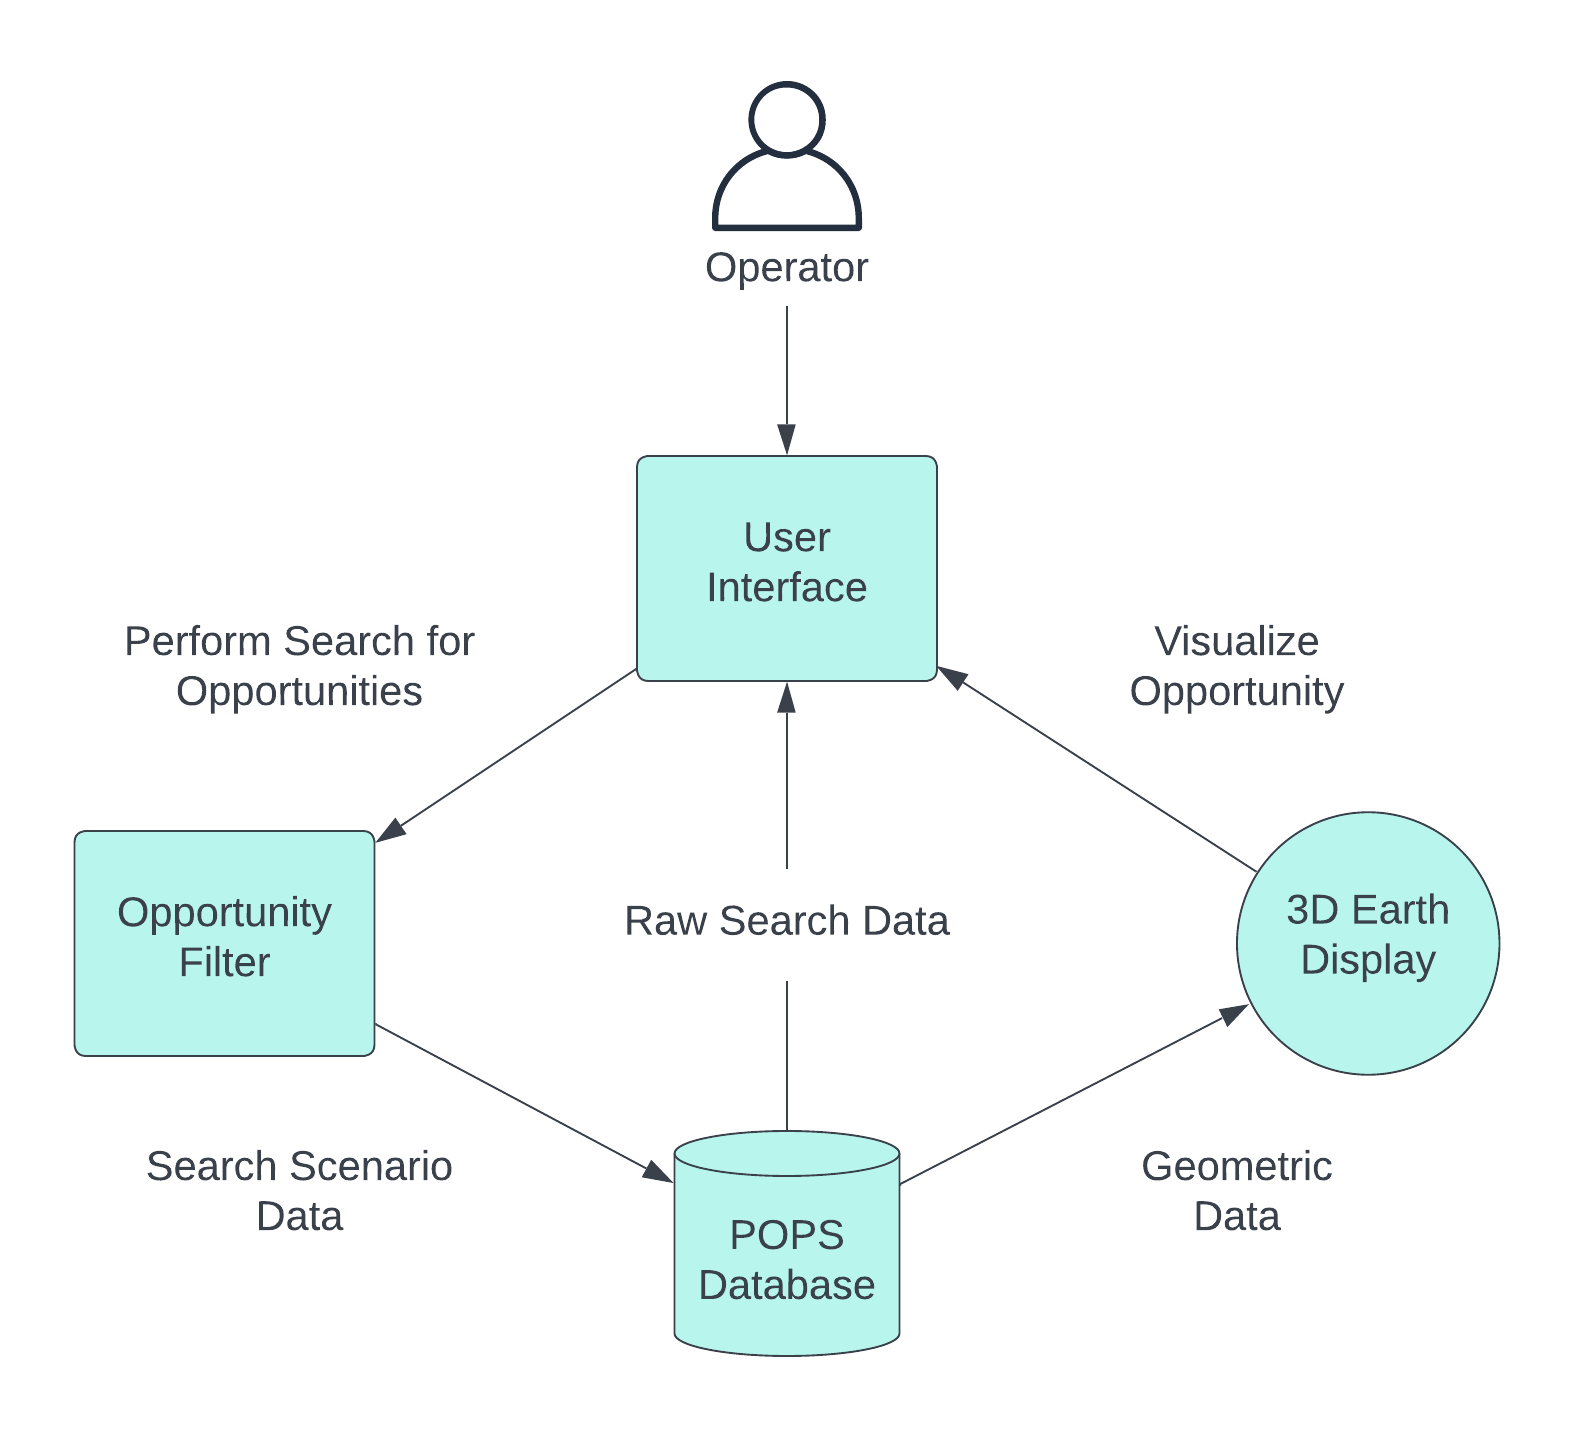
\includegraphics[width=0.5\textwidth]{opp_search_flow.png} 
    \caption{Observation Filtering Summary}
    \label{fig:obs_fil} 
\end{figure}

Once our scenario is set up, we begin Observation Configuration. \gls{pops}
must display potential observation opportunities to the user and must enable
the user to create observations based on these potential opportunities.
Opportunity filtering is the process of taking a large set of potential
observations and constraining them to an \gls{aoi}. Observations can be
performed anywhere on Earth, but we only care about those that provide useful
data for our operations strategy.  The basic process for displaying
opportunities to the user can be seen in Figure~\ref{fig:obs_fil}. An operator
first creates a search scenario through the \gls{gui}.  For a given mission,
there may be multiple observation types, multiple possible \glspl{aoi}, and a
combination of one or more satellites that are part of the observation. All of
this is specified by the user in the form of a search scenario. These
parameters are fed to the Opportunity Filter which generates search data.
Rather than having the search data displayed immediately, all of the generated
search data is stored in the database. From here, it can be retrieved at any
time, without needing to re-compute a search scenario. Some raw search data may
be retrieved and displayed directly. Mostly, these are just access times.
Alternatively, the raw data may undergo further processing to be displayed in
the 3D Earth visualization. Currently, satellites, satellite trajectories,
ground stations, ground access times, \glspl{aoi}, and swaths can be displayed.


Since an operator will spend most of their time on the Observation
Configuration page, we shall spend some time discussing it and the utilities
provided with the page. It should be emphasized that \gls{gui}  development is
difficult and time-consuming. A good \gls{gui} and a bad \gls{gui} can
functionally do the same thing but the good \gls{gui} will be easier to use,
robust, and visually pleasing. What's more is that they are extremely
time-consuming; hours can be spent on just a single button, for example. The
goal for \gls{pops} is not to create the perfect user interface but rather the
actual functionality itself, time spent on the webpages themselves is minimized
in favor of creating a functional product. 

\begin{figure}
    \centering
    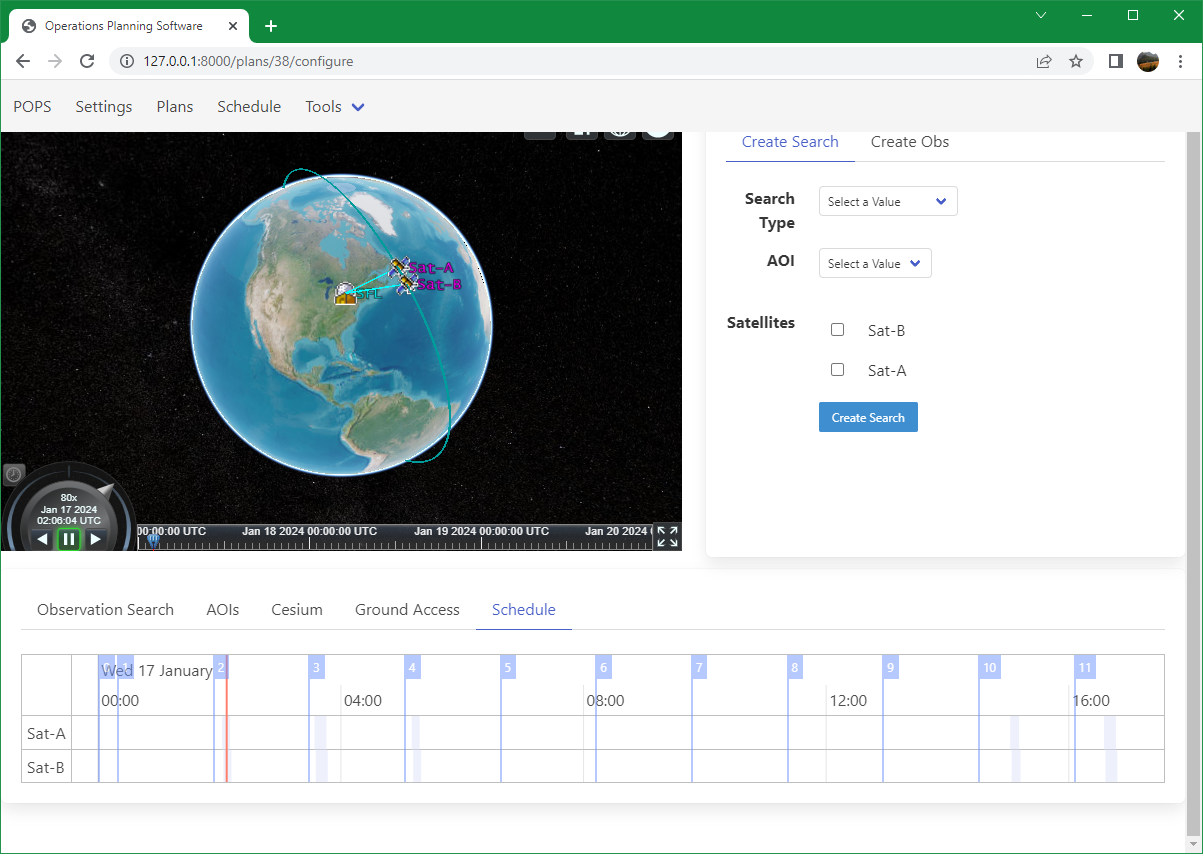
\includegraphics[width=0.8\textwidth]{obs-conf-base.png} 
    \caption{Observation Configuration Webpage}
    \label{fig:obs-conf-base} 
\end{figure}


With that in mind, the Observation Configuration page can be seen in
Figure~\ref{fig:obs-conf-base}. The Cesium viewer is located on the top left of
the page.  There, an operator can see: the Earth, the satellites, their
trajectories, possible ground access times, an Area of Interest, and potential
observation opportunities. In the top right are forms that the user can fill
out to add or make changes to the plan. Currently, that consists of forms to
create search scenarios or to add observations to the plan. The bottom tabs are
meant to display information to the user or allow them to interact with the
Cesium viewer. Currently visible, in the bottom is the schedule timeline.
Here, events are displayed to the user in an interactable viewer.

To create a search, a user must specify the search type, the \gls{aoi} the
search should be conducted on, and the  satellites that should be considered.
When the \texttt{Create Search} button in clicked, \gls{pops} will send the
data to the Opportunity Filter and a search will be performed. The observation
creation tab is under developed and only contains a placeholder form currently.

\begin{figure}
    \centering
    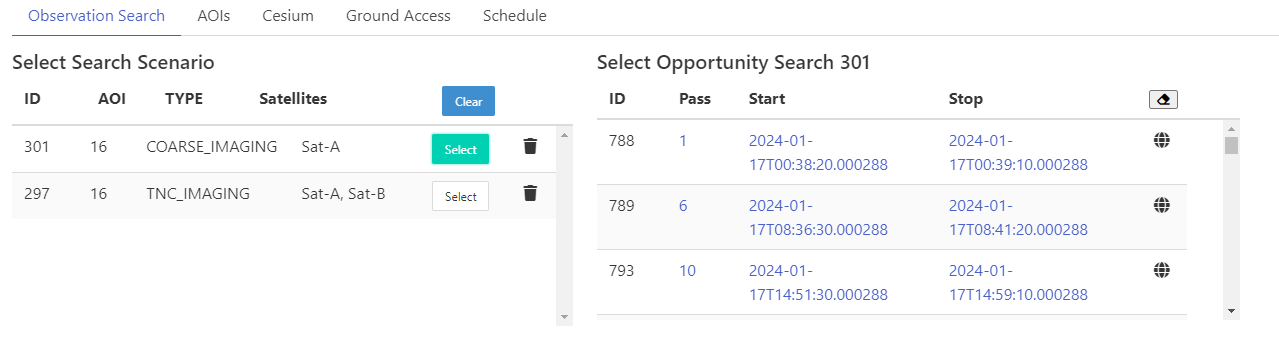
\includegraphics[width=0.8\textwidth]{obs-conf-search.png} 
    \caption{Observation Search Tab}
    \label{fig:obs-conf-search} 
\end{figure}

The results of the search can be seen in the observation search tab in
Figure~\ref{fig:obs-conf-search}. This tab is split into two lists. The left
list displays a list of the search scenarios that are associated with the plan.
When a new search scenario is added, it is added to this list. Here, search
scenarios can be deleted with the trash icon or they may be displayed in the
viewer. For a selected search scenario, the right list displays all of the
opportunities associated with it. Information such as the pass index of the
opportunity, start epoch and end epochs are displayed to the user. The blue
text entries are hyperlinks. When clicked, they update the current time of the
Cesium viewer. For example, for opportunity \texttt{788} (these are global IDs
not search scenario IDs) if the user clicks on the start epoch, the viewer will
change time to 12:38 AM Jan 17, 2024. The globe icon on the right allows a user
to display or hide an opportunity. Similarly, the eraser icon in the header
toggles the visibility of all opportunities.  The usefulness of these can be
seen in Figure~\ref{fig:obs-conf-opps}.  In Figure~\ref{fig:obs-conf-opps-1},
all of the opportunities in the scenario are displayed. This is of course quite
messy and difficult to understand. In Figure~\ref{fig:obs-conf-opps-2} all of
the opportunities in the scenario have been hidden except for two
opportunities. This makes it far easier to select only the opportunities that
are of interest to an operator.


\begin{figure}[h] 
    \centering
    \begin{subfigure}[b]{0.49\textwidth}
	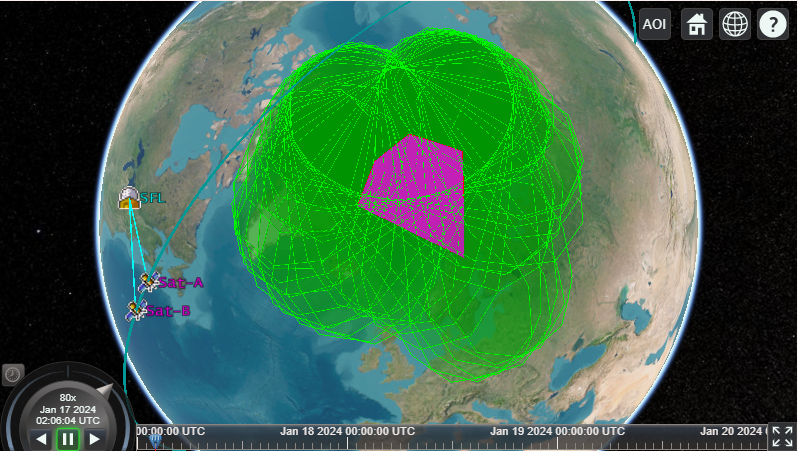
\includegraphics[width=\textwidth]{obs-conf-ces-coarse-1.PNG} 
	\caption{All Opportunities}
	\label{fig:obs-conf-opps-1} 
    \end{subfigure}
    \hfill
    \begin{subfigure}[b]{0.49\textwidth}
	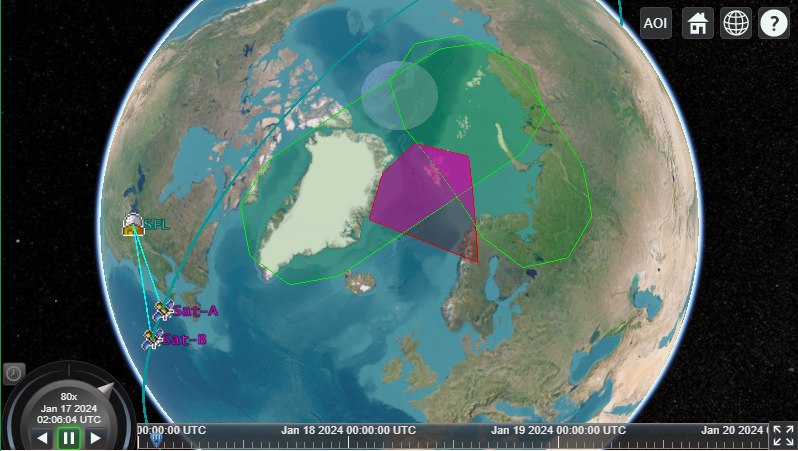
\includegraphics[width=\textwidth]{obs-conf-ces-coarse-2.PNG} 
	\caption{Two Opportunities}
	\label{fig:obs-conf-opps-2} 
    \end{subfigure}
    \caption{Opportunities Displayed in Cesium}
    \label{fig:obs-conf-opps} 
\end{figure}

Every \gls{aoi} that is stored in \gls{pops} can be seen in the \texttt{AOI}
tab. \gls{aois} May be added either through a text file that is read and loaded
into \gls{pops}. Alternatively, \glspl{aoi} can be draw directly in the Cesium
viewer with the \texttt{aoi} button in the Cesium viewer. When it is clicked,
the controls for the viewer change. Every time a user clicks on the Earth, a
polygon vertex is placed at that location. As vertexes are added a white
polygon becomes visible. If a mistake is made, the user can undo vertices by
pressing \texttt{CTRL-Z}. To give the user more information, some instructions
are included in a text box as well as the Latitude and Longitude of the cursor.
Once the user is satisfied, they can right click and the area-target \gls{aoi}
is saved to the database and can be referenced by search scenarios. A Partially
completed \gls{aoi} can be seen in Figure~\ref{fig:obs-conf-draw}.

\begin{figure}[h]
    \centering
    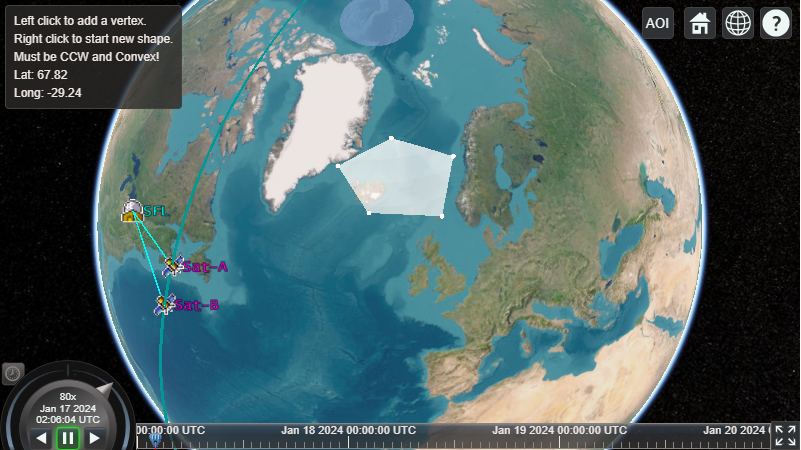
\includegraphics[width=0.8\textwidth]{obs-conf-draw.png} 
    \caption{Drawing an AOI}
    \label{fig:obs-conf-draw} 
\end{figure}

The last two tabs serve minor purposes. The \texttt{Cesium} tab lists all of
the currently loaded objects in the Cesium Viewer. It allows a user to display
or hide any object. This is mostly useful for debugging, or if a user wants a
specialized view. For example, they may wish to show the intersection polygons
from a number of opportunities. Alternatively, they may wish to compare swaths
from different passes. This tab gives the user the granular ability to make
those changes. The \texttt{Ground Access} tab shows a filter-able list of
ground station accesses, with time links that change Cesium's current time.

\subsection{Scheduling}


Once observations are added to a plan, they must be added to the schedule and
validated. The schedule is universal to any observation, plan, or mission and
is used to describe what actions a satellite may perform. For this reason, it
is a separate part of the software. The schedule is contained and interacted
with via the scheduler class. With it, events may be added, removed, edited, or
queried for. An event describes an action or a series of actions that a
spacecraft might make within some time range. It is a general object that can
be used to describe any arbitrary item in the schedule. Observations, attitude
maneuvers, ground station contacts, or propulsive maneuvers are examples of
potential events. Even though \gls{pops} is intended to only handle payload
operations and not other types of orbit operations, it is still important for
an operator to be aware of what other events are planned for a particular
satellite in case there is a conflict. Another aspect of events to note is that
they may be linked together. This is necessary for situations where there are
multiple events associated with a single observation. This is the case when
multiple satellites are used for an observation or there is some time between
actions.  

Events may be added through the observation configuration page or an interface
with \gls{sfl}’s other ground support software. If \glspl{ttc} have been
uploaded to the satellite, they are visible in the schedule. Once added, events
are immediately stored in the database. Events can be visualized either in
tabular form or displayed graphically with an interactable timeline. The
timeline allows for scrolling and zooming and also allows the user to edit or
delete events. Not all events may be relevant to a user when they are
constructing a plan, so events are filtered based on relevance. For example,
only observations within the plan’s time range are displayed.

Finally, once events are added to the schedule, the schedule is then validated.
Validation is based off of a library of validation rules. All events are
evaluated with each rule and any conflicts are logged. Currently, only one rule
has been implemented; that being: no two events may happen simultaneously on
the same satellite. More rules will be added such as: observation specific
rules (a plan must conform with a satellite’s data budget), attitude control
considerations, as well as the weather forecast. Again, \gls{pops} is meant to
be an easily generalizable tool, so rules may be added as necessary.


%\begin{figure}[h] 
%    \centering
%    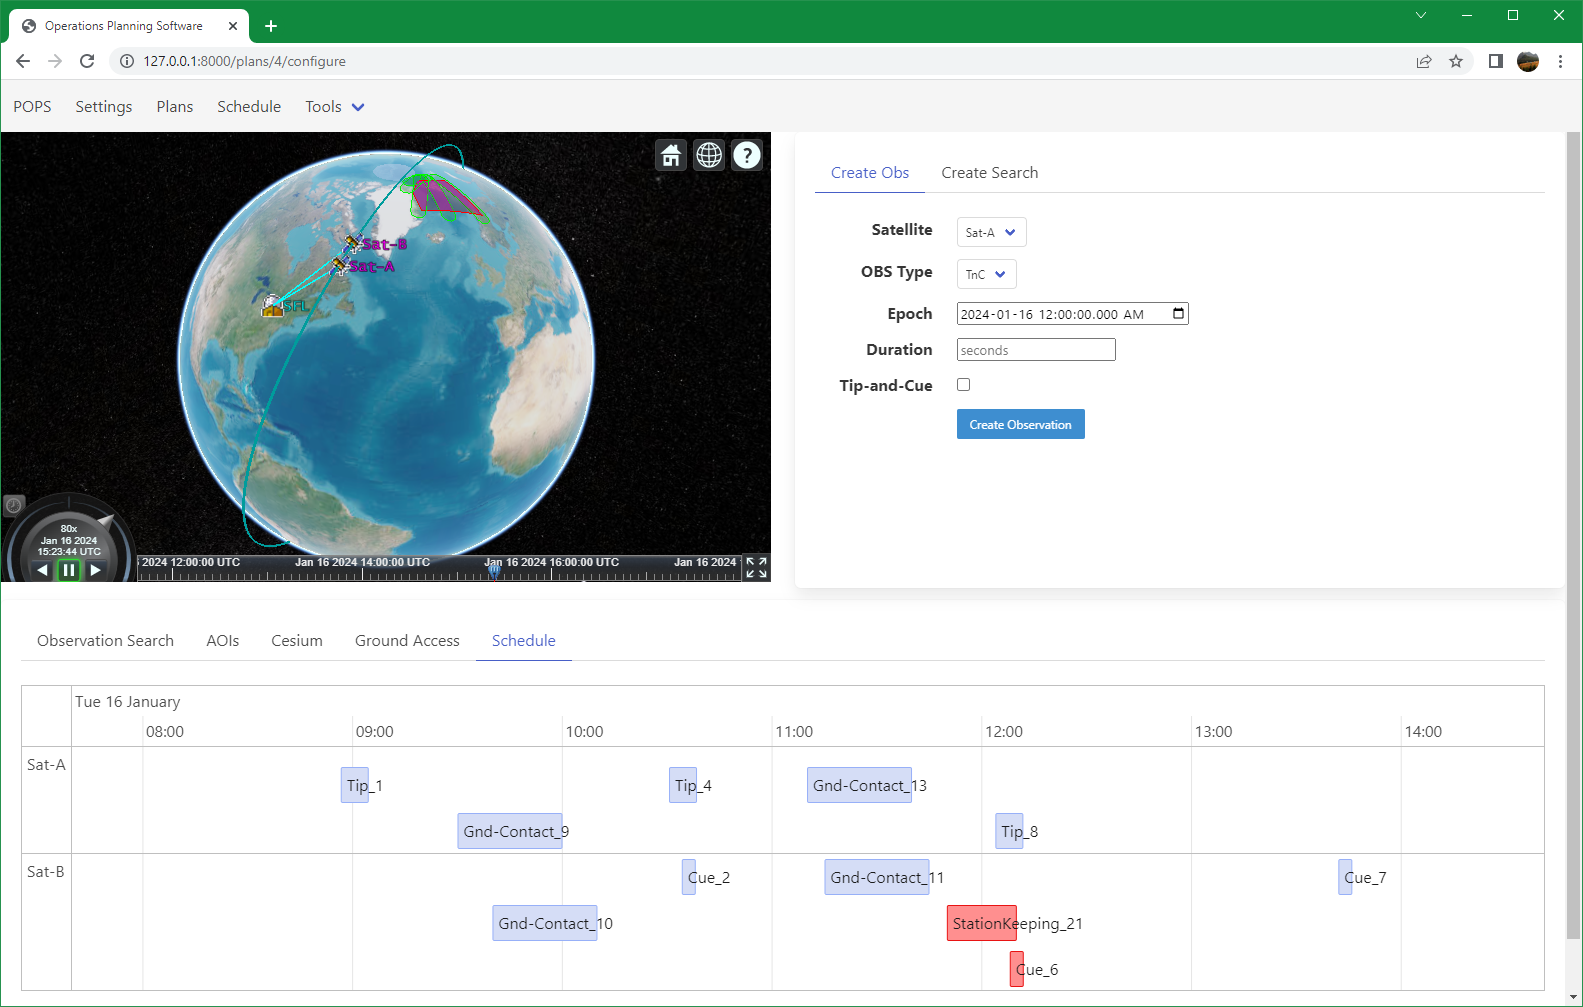
\includegraphics[width=\textwidth]{2023-04-05-POPS-1.PNG} 
%    \caption{Screenshot of Observation Configuration Page}
%    \label{fig:screen-1} 
%
%    \includegraphics[width=\textwidth]{2023-04-05-POPS-LABELS.PNG} 
%    \caption{Labeled Screenshot of Single Opportunity}
%    \label{fig:screen-2} 
%\end{figure}
%
%\begin{figure}[h] 
%    \centering
%    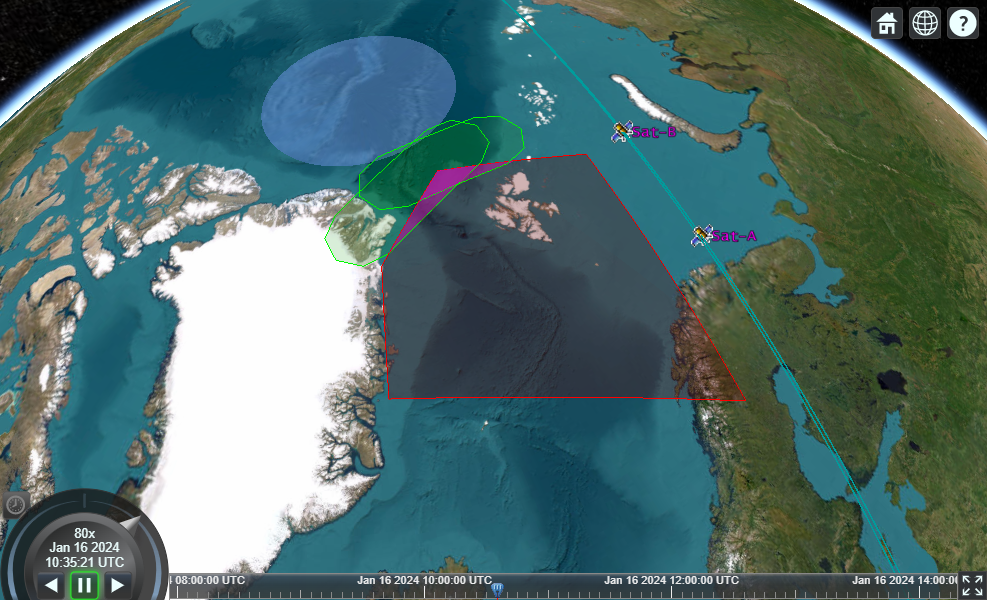
\includegraphics[width=\textwidth]{2023-04-05-POPS-4.PNG} 
%    \caption{Good Quality Observation Opportunities}
%    \label{fig:screen-3} 
%
%    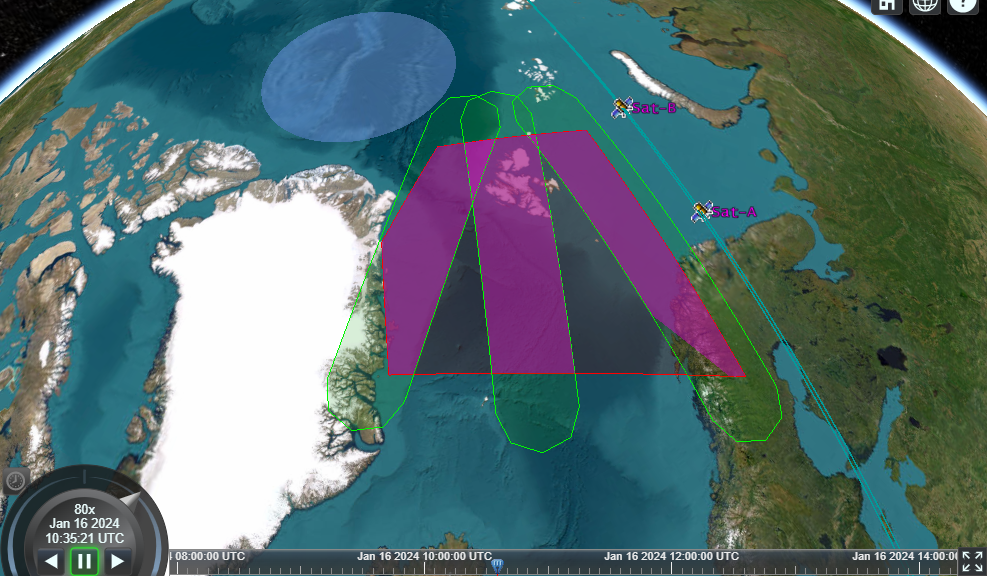
\includegraphics[width=\textwidth]{2023-04-05-POPS-5.PNG} 
%    \caption{Poor Quality Observation Opportunities}
%    \label{fig:screen-4} 
%\end{figure}


Figure \ref{fig:screen-2}, shows a close-up labeled screenshot of the 3D Earth
viewer.  Here, the \gls{aoi} is represented as a dark polygon with a red
outline, Sat-A and Sat-B’s swaths are visualized in green, and finally, the
intersection polygon is displayed in magenta. For this labeled diagram, the
first-pass ‘Tip’ swath of Sat-A is visualized. This is not done for the
following figures to avoid visual clutter. Also, notice how the intersection
polygon is the intersection area of Sat-A’s swath, Sat-B’s swath, and the
intersection polygon. Part of the purpose of POPS is to enable an operator to
judge the quality of a potential observation. It is clear that the
opportunities in Figure \ref{fig:screen-3} are good quality because they
observe large portions of the \gls{aoi}. The opportunities in Figure
\ref{fig:screen-4} are less desirable because they barely clip the AOI and have
very short access times.


\subsection{Time-Tag Command Generation}

The last stage of the \gls{pops} workflow is \gls{ttc} generation.  At this
point, the operator has created a plan that suits their own needs as well as
their customer’s needs, the plan has been validated, and all that remains is
generating \glspl{ttc} to be uploaded to their specific spacecraft.  Depending
on the observation mode, not all events have commands to be generated. In our
‘EG-SAT’ example case, on the first pass, we may command the satellite to begin
capturing wide-view images. But, on the next pass, we cannot command the
satellite to image potential targets as we cannot know where they will be a
priori. It is known that new commands will be generated between the first and
second pass and, from a planning perspective, this is handled with the
scheduler. The time when these inter-pass commands will be executed will lie
within the second-pass event. In this way, no other \glspl{ttc} should conflict
with the automatically generated commands because if they were scheduled for
that time, they would conflict. 

To generate \glspl{ttc}, templates are combined and populated based on the
observation and the configuration parameters specified when creating the
observation. For example, one parameter may be the duration for which Sat-A
captures images. This value would then be set to an offset parameter in the
templates. 

\begin{figure}[h] 
    \centering
    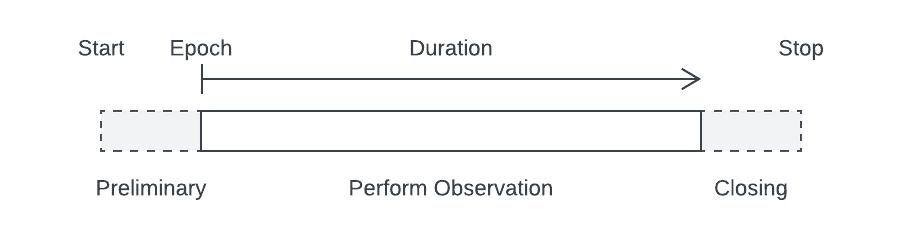
\includegraphics[width=0.7\textwidth]{timing_diagram.png} 
    \caption{Timing Diagram}
    \label{fig:timing} 
\end{figure}

The generation process is fairly straightforward and specific to each
observation mode on each satellite. But, there are some intricacies worth
noting. Firstly, from the previous example, when creating an observation, the
operator only specifies a duration because that is all they are concerned with.
Generally, for any observation, there are some preliminary and closing
commands. These commands cannot happen instantaneously and may require some
non-negligible margin. It is for this reason that each event is subdivided into
separate timing components. This can be seen in Figure \ref{fig:timing}. The
start and stop times are the same as the event’s start and stop but they
specify when the first \gls{ttc} is executed and when the final \gls{ttc} has
concluded its execution respectively. The epoch is the time when the
observation begins sensing and the duration is the period after which the
sensing is performed. As part of the \gls{ttc} generation capabilities, these
timings can be determined programmatically by evaluating the templates for each
observation. As such, when an observation is created by the operator in the
observation configuration stage, they specify the epoch and the duration, and
the \gls{ttc} generator determines the start and stop times.





